\chapter{UWB Handling}

\section{Distance Measurement}
The distance measurements in this system are conducted using a Time-of-Flight (ToF) methodology. This means that the time taken for an Ultra-Wideband (UWB) message to be transmitted from one device and received by another is a crucial factor. By subtracting the time when the UWB message is transmitted from the time it is received, we obtain the flight time. This represents the duration it took for the electromagnetic field to propagate from the sender to the receiver. This time is typically measured in seconds.
\vspace{4pt}
\newline
To derive the distance between the two UWB devices, this time is multiplied by the approximate velocity at which these electromagnetic fields expand. In a perfect vacuum, this velocity would equal the speed of light, which is 299,792,458 meters per second, often denoted as 'c'. However, under atmospheric conditions where this setup operates, the speed of light is slightly slower. Therefore, in this setup, an approximated speed of 299,702,547 meters per second is used. 
\vspace{4pt}
\newline
It's worth noting that the accuracy of the time measurement is crucial since even a small error in this time measurement can result in a relatively significant error in distance estimation. To ensure precise time measurements, the DW3000 IC requires a highly accurate clock signal with minimal drift. The DWM3000 module offers an advantage in this regard, as it already integrates the DW3000 chip with an on-module oscillator suitable for UWB operations.
A visual representation of the ToF distance calculation process is depicted in Figure \ref{fig:tof_sketch}.

\begin{center}
	\begin{figure}[!hbt]
		\centering
		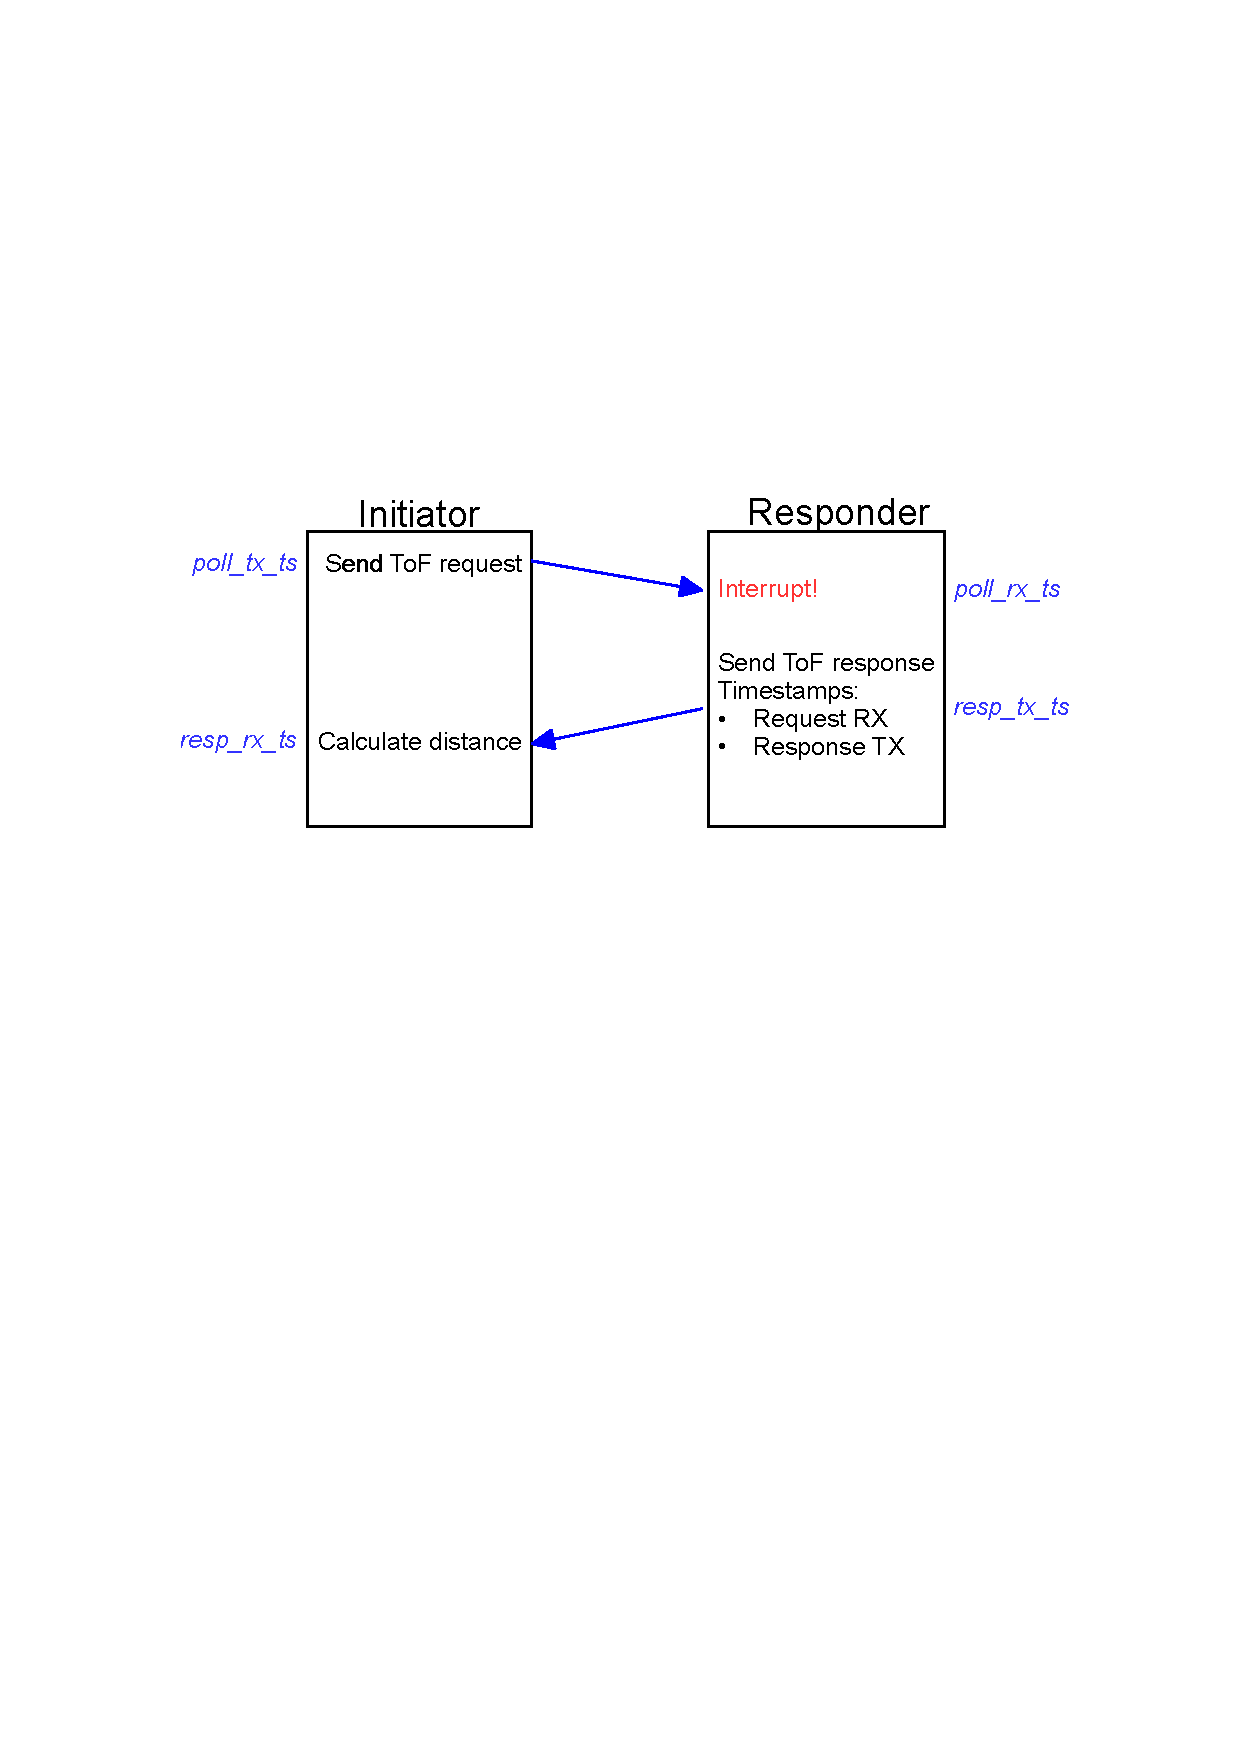
\includegraphics[width=0.8\textwidth]{pictures/ToF_scheme.pdf}
		\caption{Sketch of the complete setup.}
		\label{fig:tof_sketch}
	\end{figure}
\end{center}


To estimate the distance, four timestamps, marked in blue in Figure \ref{fig:tof_sketch}, are used. These timestamps are expressed in ticks and are stored in a 32-bit variable. The timestamps are as follows:

\begin{center}
	\begin{table}[!hbt]
		\begin{tabular}{ | m{5em} | m{10cm} |} 
			\hline
			poll\_tx\_ts & Time of request being sent by Initiator \\ 
			\hline
			poll\_rx\_ts & Time of request being received by Responder \\ 
			\hline
			resp\_tx\_ts & Time of response being sent by Responder \\ 
			\hline
			resp\_rx\_ts & Time of response being received by Initiator \\ 
			\hline
		\end{tabular}
		\caption{Timestamp variables.}
		\label{tab:timestamps}
	\end{table}
\end{center}

To calculate the time it took for the poll message to travel from the initiator to the responder, the \blueconsolas{poll\_tx\_ts} timestamp is subtracted from the \blueconsolas{poll\_rx\_ts} timestamp, yielding the \blueconsolas{rtd\_init} value. Similarly, for the time the response message took to travel in the opposite direction, \blueconsolas{resp\_tx\_ts} is subtracted from \blueconsolas{resp\_rx\_ts}, resulting in the \blueconsolas{rtd\_resp} variable.
\vspace{4pt}
\newline
To determine the distance between the initiator and the responder, the two times (\blueconsolas{rtd\_init} and \blueconsolas{rtd\_resp}) are averaged. Before averaging, the response time (\blueconsolas{rtd\_resp}) is adjusted by applying an offset factor (1 - clockOffsetRatio). This compensates for potential variations that may arise if the clock of the initiator runs slightly faster or slower than the responder due to factors such as aging effects, temperature, voltage, or manufacturing discrepancies.
\vspace{4pt}
\newline
Finally, to compute the distance between the two devices, the average time is converted to seconds and then multiplied by the predefined speed of light, representing the speed of electromagnetic field expansion.
\vspace{4pt}
\newline
This process is subsequently repeated for all of the saved anchors to get the distance to every single one. 
The calculated distances are savced in the distances array in the 



\section{Transmission of CSI}

\section{Watchdog Handling}


